\section*{Dati e risultati}

\subsection*{Ponte di Wien}

L'oscillatore a ponte di Wien si può realizzare seguendo lo schema circuitale riportato in Figura \ref{fig:oscillatore}.
Il circuito è quindi costituito da un amplificatore operazionale UA741 che presenta due due reti di retroazione, una positiva e una negativa.

Analizziamo inizialmente la rete di retroazione positiva e il suo effetto sulla tensione di output $V\ped{out}$.
Questo ramo di retroazione è formato da una resistenza $R_2$ in serie ad un condensatore $C_1$, quindi possimo dire che sia un filtro passa alto. Questo primo blocco avrà un'impedenza $Z_4$. L'ingresso non invertente $V^+$ è collegato al comune mediante un parallelo tra una resistenza $R_3$ ed un condensatore $C_2$. Questo secocndo blocco avrà un'impdenza $Z_3$. Facciamo notare che $R_2=R_3=R$ e $C_1=C_2=C$.

\begin{wrapfloat}{figure}{O}{0pt}
	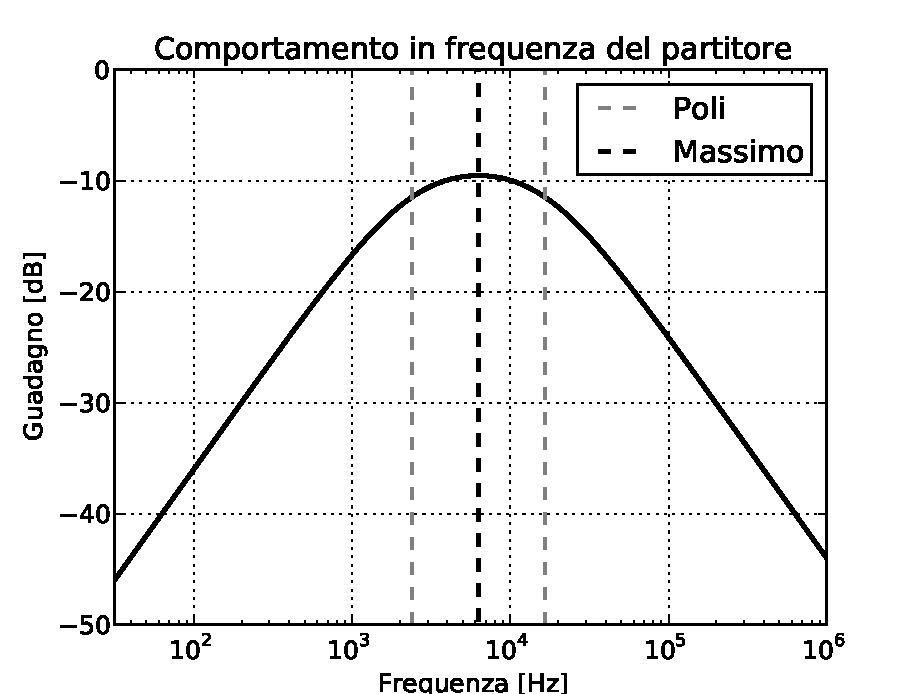
\includegraphics[width=0.5\textwidth]{figure/ctp.pdf}
    \caption{Questa immagine riporta l'andamento delguadagno $\beta$ del partitore di tensione in funzione della frequenza. Come descritto nell'analisi sopra riportata alla frequenza di picco corrisponde la condizione che la tensione in uscita dall'oscillatore sia esattamente 1/3 della tensione in ingresso allo stesso.}
    \label{fig:guadagno_partitore}
\end{wrapfloat}

Quindi grazie al calcolo delle impedenze, analizzando singolarmente la struttura del ramo di retroazione positiva, possiamo trovare la funzione di trasferimento di questo piccolo circuito. Ovvero:
\begin{equation}
	Z_3\,=\,\frac{R}{1 + i \omega C R} \qquad \text{e} \qquad Z_4\,=\,R + \frac{1}{i \omega C}
\end{equation}
dove abbiamo indicato con $R$ le resistenze $R_2\,=\,\SI{10}{\kilo\ohm}$. Quindi otteniamo che:
\begin{equation}
	V\ped{O}\,=\,\frac{Z_3}{Z_3 + Z_4} \cdot V\ped{I}\,=\,\frac{i \omega R C}{(1 + i \omega C R)^2 + i \omega C R} \cdot V\ped{I}
\end{equation}
dove con $V\ped{O}$ abbiamo indicato la tensione in uscita da questo blocco e con $V\ped{I}$ il segnale in ingresso allo stesso.
Quindi, analizzando la funzione appena trovato ci si può rendere conto che rappresenta un filtro passa banda. Inoltre possiamo calcolare il guadagno $\beta$ della retroazione positiva:
\begin{equation}
	\beta\,=\,\frac{V\ped{O}}{V\ped{I}}\,=\,\frac{i \omega R C}{1 - (\omega C R)^2 + 3 i \omega R C}
\end{equation}
Grazie a questa relazione possiamo osservare che se la frequenza del segnale in ingresso $f$ è uguale alla frequenza di risonanza $f_0$ del circuito abbiamo che il segnale in uscita $V\ped{O}\,=\,\frac{1}{3} \cdot V\ped{I}$. Infatti la frequenza di risonanza del nostro filtro passa banda vale:
\begin{equation}
	f_0\,=\, \frac{1}{2 \pi R C} \qquad \text{con} \qquad \omega_0\,=\,\frac{1}{RC}
\end{equation}
quindi se $\omega \,=\, \omega_0$ abbiamo che:
\begin{equation}
	V\ped{O}\,=\,\frac{1}{3} \cdot V\ped{I}
\end{equation}

%\begin{wrapfloat}{figure}{I}{0pt}
%\includegraphics[width=0.5\textwidth]{Relativo}
%\caption{Esempio di figura ‘‘avvolta’’ da un testo.}
%\end{wrapfloat}

%\begin{figure*}[h]
%    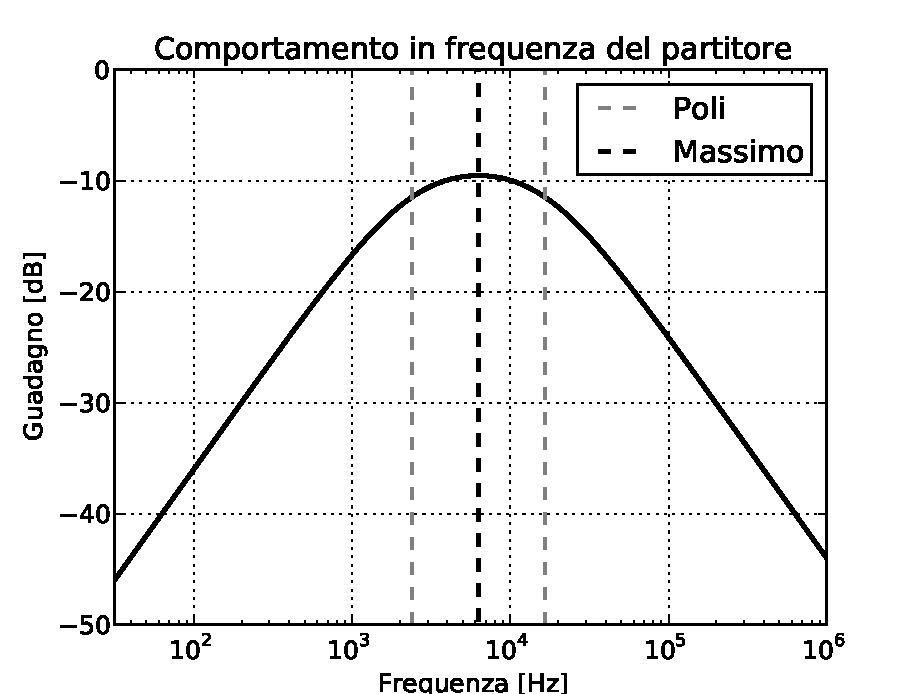
\includegraphics[height=0.35\textheight]{figure/ctp.pdf}
%    \caption{Questa immagine riporta l'andamento delguadagno $\beta$ del partitore di tensione in funzione della frequenza. Come descritto nell'analisi sopra riportata alla frequenza di picco corrisponde la condizione che la tensione in uscita dall'oscillatore sia esattamente 1/3 della tensione in ingresso allo stesso.}
%    \label{fig:guadagno_partitore}
%\end{figure*}

Quindi grazie a questo noi sappiamo che al'ingresso non invertente $V^+$ dell'amplificatore operazionale abbiamo una tensione che vale un terzo della tensione in uscita dall'amplificatore $V\ped{out}$.
Da questo risultato segue che per ottenere oscillazioni stabili nel tempo anche la tensione all'ingresso inverente $V^-$ dell'amplificatore deve valere un terzo della tensione di output.

Quindi, come nel caso precedente, se analizziamo separatamente questa parte di circuito, ovvero il ramo di retroazione negativo otteniamo che:
\begin{equation}
	A\,=\,1 + \frac{R_v}{R_1} \qquad \text{inoltre} \qquad V\ped{out}\,=\,AV^- \qquad \text{da cui} \qquad V^+\,=\,\frac{V\ped{out}}{A}
\end{equation}
pertanto visto che vogliamo che $V^+\,=\,\frac{1}{3} \cdot V\ped{out}$ si ottiene che $A\,=\,3$ e quindi:
\begin{equation}
	R_v\,=\,2R1
\end{equation}

Quindi fino ad ora abbiamo analizzato i due rami di retroazione dell'oscillatore e la condizione di stabilità del circuito, ovvero il caso in cui la frequenza di oscillazione corrisponde alla frequenza di risonanza del filtro passa banda.
Tuttavia in classe abbiamo visto che a seconda del valore del prodotto tra $A$ e $\beta$ si possono avere tre condizioni differenti della tensione in uscita dall'amplificatore.
Pertanto ora procediamo nell'analisi del prodotto:
\begin{equation}
	\left|A \cdot \beta \right|
\end{equation}
\begin{itemize}
	\item{Se $\left|A \cdot \beta \right|\,=\,1$ si ottengono delle oscillazioni di ampiezza costante nel tempo di $V\ped{out}$;}
	\item{Se $\left|A \cdot \beta \right|\, \leq \,1$ l'ampiezza dell'oscillazione di $V\ped{out}$ si smorza gradualmente;}
	\item{Se $\left|A \cdot \beta \right|\, \geq \,1$ l'ampiezza dell'oscillazione di $V\ped{out}$ aumenta man mano nel tempo fino a che la tensione di output non raggiunge i valori di saturazione positivi e negativi;}
\end{itemize}

In Figura \ref{fig:wien_instable} è raffigurato l'andamento della tensione di output $V\ped{out}$ dell'oscillatore nel caso in cui il guadagno complessivo del circuito risulti essere maggiore o minore di uno. Quindi sono i casi in cui l'uscita del circuito non è stabile.

\begin{figure*}[h]
    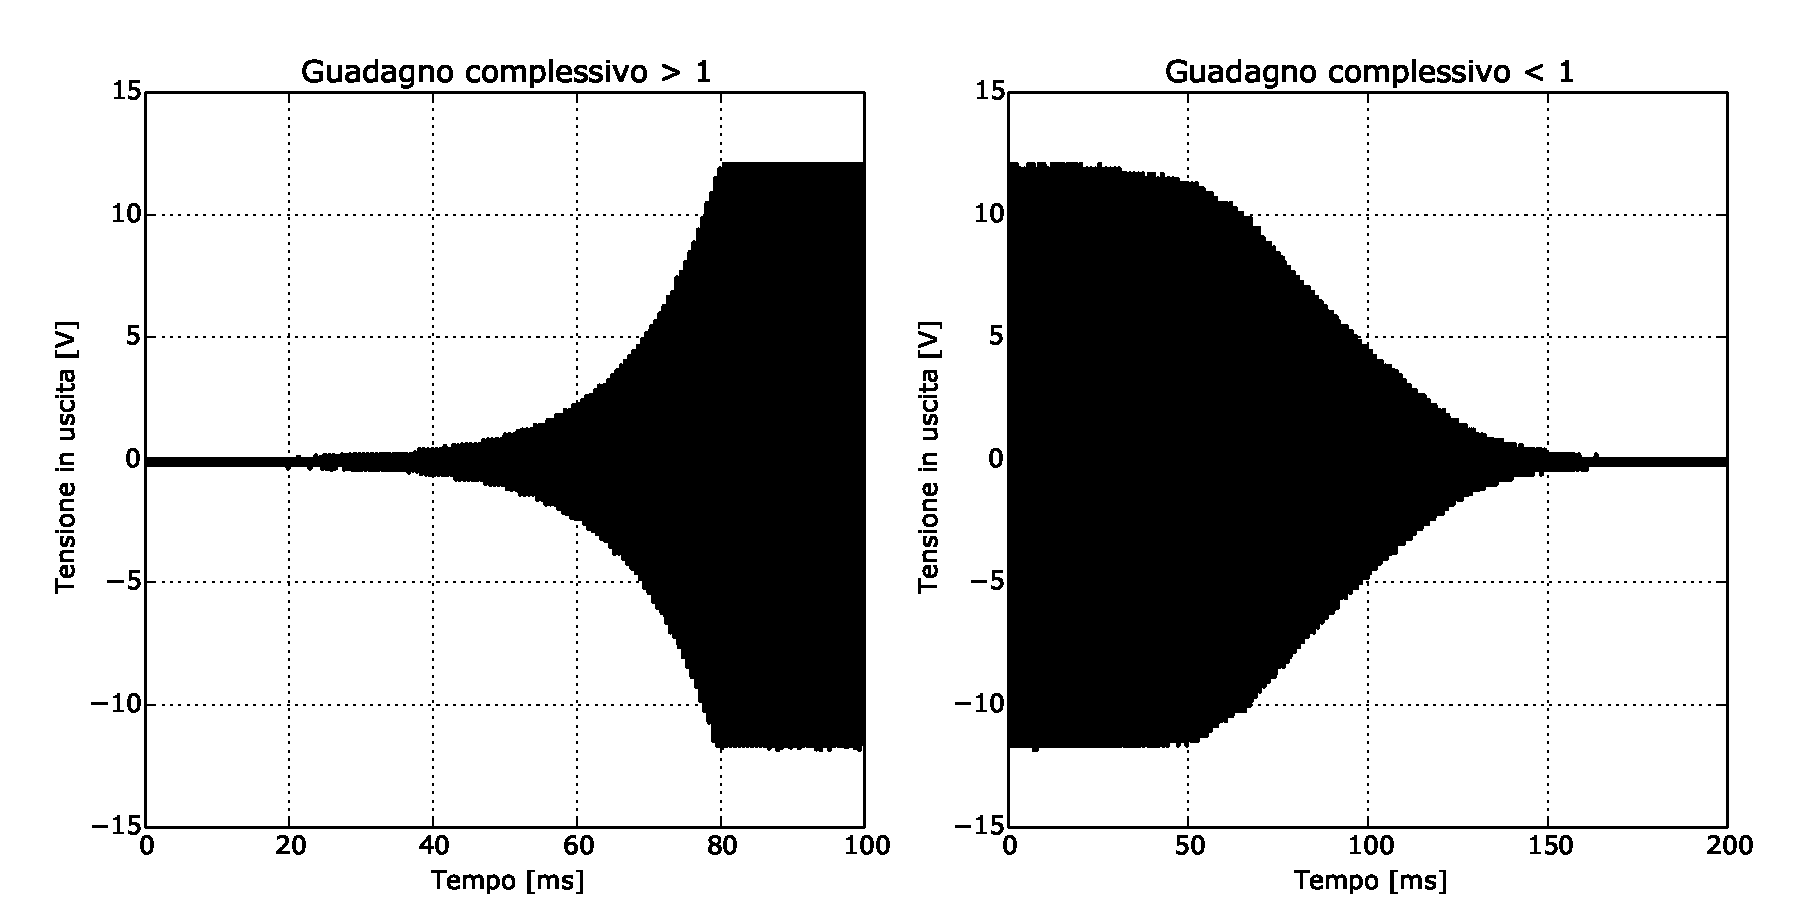
\includegraphics[height=0.35\textheight]{figure/exp_imp.pdf}
    \caption{Questa immagine riporta l'andamento della tesione in uscita dall'oscillatore in funzione del tempo. Nel grafico a sinistra è possibile osservare l'andamento di $V\ped{out}$ nel caso in cui il guadagno comlessivo del circuito risultasse maggiore di 1. Mentre nel grafico a deltra è riportato l'andamento di $V\ped{out}$ nel caso in cui il guadagno comlessivo del circuito sia minure di 1.}
    \label{fig:wien_instable}
\end{figure*}

Quindi prima di concludere questa analisi più teorica che pratica sull'oscillatore a ponte di Wien occorre illustrare come si innesca l'oscillazione di tale circuito. Questo particolare tipo di oscillatore è detto ``autoinnescante''. In pratica l'autoinnesco è reso possibile dalla presenza certa di una componente di rumore con frequenza $f_0$ nel sistema costituito dall'amplificatore e dalla rete di retroazione. Questa componenente infinitesimale viene amplificata dall'anello di retroazione positiva, trasformandosi in un'oscillazione di ampiezza elevata. Pertanto per innescare il circuito basta che sia soddisfatta la condizione che $\left|A \cdot \beta \right|\, \geq \,1$ overo che $R_v\, \geq \,2R_1$.

Tuttavia innescando in questo modo il nostro circuito ci ritroviamo nella situazione per cui $\left|A \cdot \beta \right|\, \geq \,1$ che ci porta inesorabilmente ad avere una $V\ped{out}$ che oscilla tra valori di saturazione positiva o negativa. Questo fatto ai fini pratici non è di nessun interesse. Inoltre dal momento che i valori di resistenza per due $R$ uguali, nominalmente hanno lo stesso valore, ma in pratica sono differenti, questa situazione può verificarsi anche non spontaneamente.

Pertanto cerchiamo ora di capire come bilanciare questo scompenso tra resistenze sia in modo automatico che manualmente. Se si vuole che questo processo avvenga automaticamente, senza dover agire direttamente sul circuito basta mettere in serie ad $R_1$ una lampadina. Infatti il comportamento del filamento prevede che la resistenza salga quando quest'ultimo si riscalda. Da questo punto di vista, l'uso di una lampadina è del tutto equivalente ad un termistore PTC. L'inerzia termica della lampadina permette di stabilizzare efficacemente l'ampiezza della sinusoide in uscita.
D'altro canto se si volesse agire direttamente sul circuito si può sempre usare una resistenza variabile, più precisamente un trimmer, come $R_v$. In questo modo è possibile innescare i circuito creando uno scompenso tra i valori di $R_v$ e $2R_2$ in modo che $\left|A \cdot \beta \right|\, \geq \,1$ e successivamente, regolando $R_v$, si porta l'oscillatore ad una situazione di stabilità imponendo la condizione $R_v\,=\,2R_2$.

Nel nostro caso abbiamo deciso di andare sul sicuro e abbiamo deciso di adottare entrambe le soluzioni, ovvero abbiamo collegato in serie alla resistenza $R_1$ una lampadina da \SI{12}{\volt} ad una corrente di \SI{50}{\milli\ampere} e abbiamo usato, come $R_v$, un trimmer.

Quello che abbiamo osservao è riportato in Figura \ref{fig:wien_stab}

\begin{figure*}[h]
    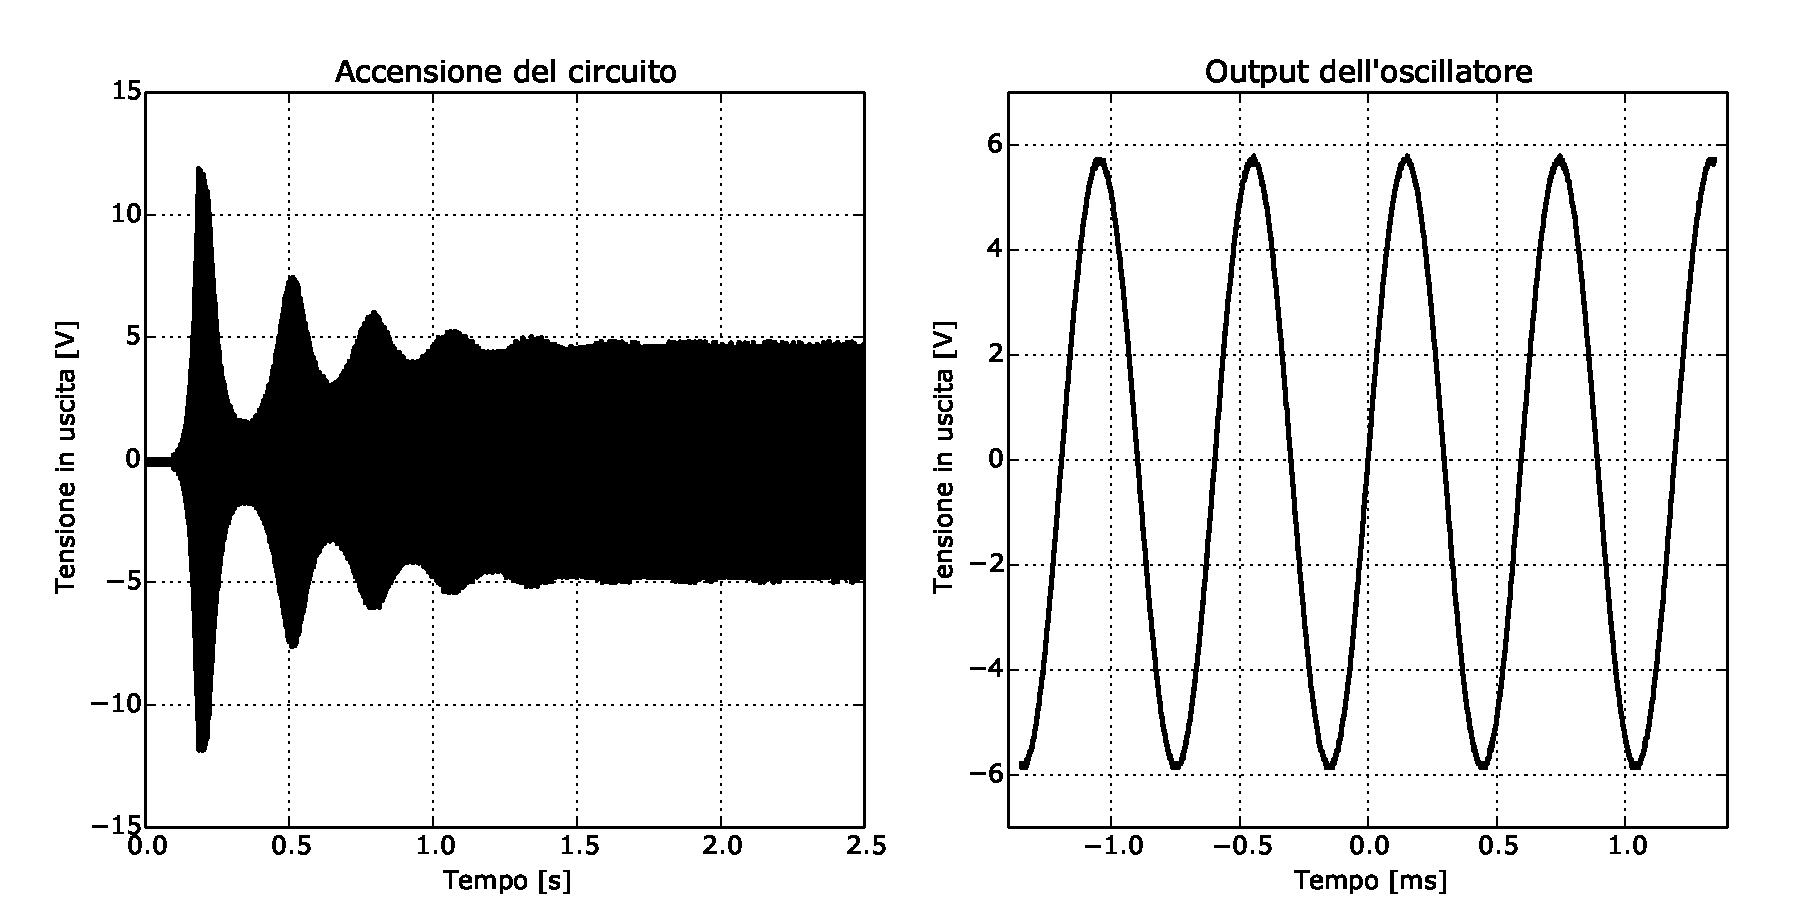
\includegraphics[height=0.35\textheight]{figure/stab.pdf}
    \caption{Questa immagine riporta l'andamento della tesione in uscita dall'oscillatore in funzione del tempo. Nel grafico a sinistra è possibile osservare l'andamento di $V\ped{out}$ dall'accensione del circuito in poi. Purtroppo non siamo in grado di spiegare la causa delle fluttuazioni dei $V\ped{out}$. Inoltre è possibile oservare che dopo circa \SI{1.5}{\second} le fluttuazioni si stabilizzano e l'ampieza delle oscillazioni si stabilizza ad un valore costante. Questo risultato è visibile nel grafico a destra che riporta l'andamento della tensione in uscita dall'oscillatore nel caso in cui il guadagno complessivo risulti essere uguale ad 1. In questo caso si può chiaramente osservare il motivo per cui tale circuito sia definito oscillatore, la frequenza e l'ampiezza delle oscillazini risultano essere costanti. In particolare abbiamo una frequenza di $(1675 \pm 5) \si{\hertz}$.}
    \label{fig:wien_stab}
\end{figure*}

\subsection*{Sonda}

Per concludere vogliamo analizzare e capire per quale motivo alcune sonde necessitano o hanno la possibilità di essere compensate. Per prima cosa facciamo riferimento al circuito riportato in Figura \ref{fig:circ_sonda} per comprendere lo schema circuitale dell'insieme sonda e oscilloscopio. Possiamo notare che come per tutti gli apparati elettronici per entrambi gli strumenti è presente una resistenza in parallelo con una capacità. Per l'oscilloscopio abbiamo $C_2//R_2$ mentre per la sonda $C_1//R_1$. A questo punto, al fine di analizzare la funzione di rasferimento del circuito, ci conviene sfruttare il concetto di impedenza. Otteniamo quindi:

\begin{equation}
	Z_1\,=\,\frac{R_1}{1 + i \omega C_1 R_1} \qquad \text{e} \qquad Z_2\,=\,\frac{R_2}{1 + i \omega C_2 R_2}
\end{equation}

dove con $Z_1$ abbiamo indicato l'impedenza della sonda, mentre con $Z_2$ quella dell'oscilloscopio. Pertanto ora il sistema risulta un banale partitore di tensione la cui funzione di trasferimento $H\ped{(\omega)}$ ha la forma seguente:

\begin{equation}
	H\ped{(\omega)}\,=\,\frac{V\ped{out}}{V\ped{in}}\,=\,\frac{Z_2}{Z_1+Z_2}\,=\,\left(\frac{Z_1}{Z_2} +1\right)^{-1}\,=\,\left(\frac{R_1\,(1 + i \omega C_2 R_2)}{R_2\,(1 + i \omega C_1 R_1)} +1 \right)^{-1}
\end{equation}
\\

\begin{wrapfloat}{figure}{I}{0pt}
	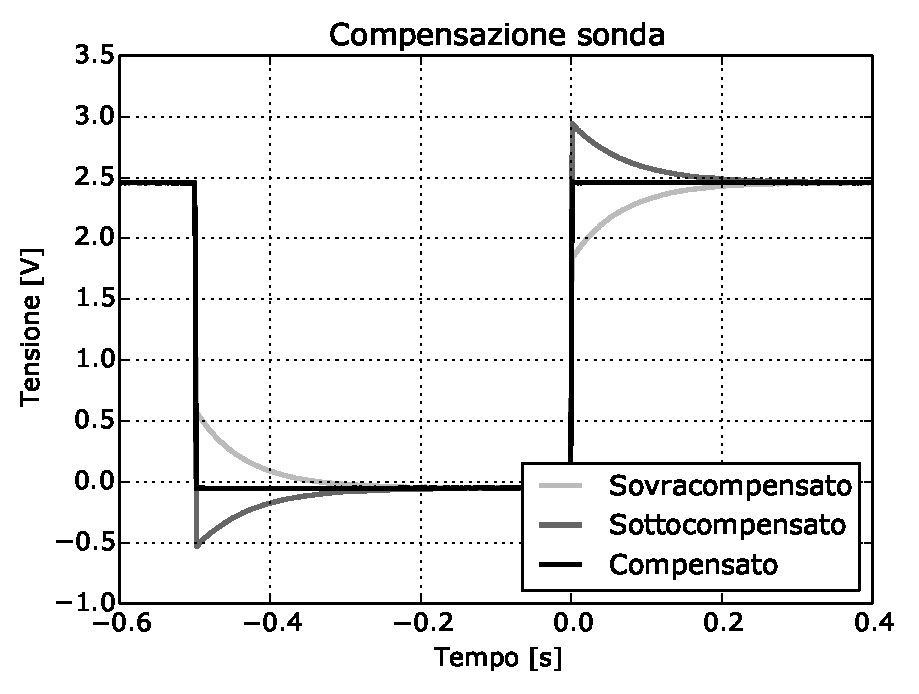
\includegraphics[width=0.6\textwidth]{figure/comp.pdf}
	\caption{Input dell'oscilloscopio con una sonda compensabile. Cambiando capacità si può ottenere una sottocompensazione, una sovracompensazione oppure compensare perfettamente le capacità, ottenendo un'onda quadra.}
	\label{fig:compensazione}
\end{wrapfloat}

dove con $V\ped{in}$ abbiamo indicato il segnale in ingresso all circuito, mentre con $V\ped{out}$ abbiamo indicato il segnale in uscita dal circuito. Quindi come si può osservare la funzione di trasferimento presenta una dipendenza dalla frequeza del segnale considerato. Pertanto per fare in modo che la sonda risulti come invisibile, ovvero che riproduca con esattezza il segnale in ingresso senza attenuarlo o amplificarlo a seconda della frequenza basta imporre la condizione per cui: $C_2 R_2=C_1 R_1$. In questo modo si eliminano i contributi dipendenti dalla frequenza e si ottiene che la funzione di trasferimento dipende solamente dai valori di resistenza $R_1$ e $R_2$.
Per questo motivo molte sonde presentano una vite di compensazione che permette di regolare il valore della loro capacità ($C_1$) al fine di soddisfar la richiesta che $C_2 R_2=C_1 R_1$ dal momento che i valori di resistenza sono fissati.

\begin{figure}[]
    \centering
    \begin{circuitikz}
        \draw
            (0, 0) node[rground] {}
            to (0, 1) to (1, 1)
            to [R, l_=$R_2$] (1, 3)
            to (0, 3) to (0, 4) to (1, 4)
            to [R, l_=$R_1$] (1, 6)
            to (0, 6)
            to [short, -o] (0, 7)
            node[anchor=east] {$V\ped{in}$}
            (0, 1)
            to (-1, 1)
            to [C, l=$C_2$] (-1, 3)
            to (0, 3)
            (0, 4)
            to (-1, 4)
            to [C, l=$C_1$] (-1, 6)
            to (0, 6)
            (0, 3.5)
            to [short, -o] (2, 3.5)
            node[anchor=west] {$V\ped{out}$}
        ;
        \draw [decorate,decoration={brace,amplitude=10pt},xshift=-4pt,yshift=0pt]
            (-2, 0.5) -- (-2, 3.4) node [black,rotate=90,midway,yshift=0.7cm] 
            {\small Oscilloscopio}
        ;
        \draw [decorate,decoration={brace,amplitude=10pt},xshift=-4pt,yshift=0pt]
            (-2, 3.6) -- (-2, 6.5) node [black,rotate=90,midway,yshift=0.7cm] 
            {\small Sonda}
        ;
    \end{circuitikz}
    \caption{Schema circuitale del sistema oscilloscopio + sonda. Il nostro oscilloscopio riporta
        i dati $R_2 = 1$ \si{\mega\ohm} e $C_2 = 12$ pF.}
    \label{fig:circ_sonda}
\end{figure}

Quanto abbiamo ottenuto è illustrato nel grafico riportato in Figura \ref{fig:compensazione}.

%\begin{figure}[t!]
%    \centering
%    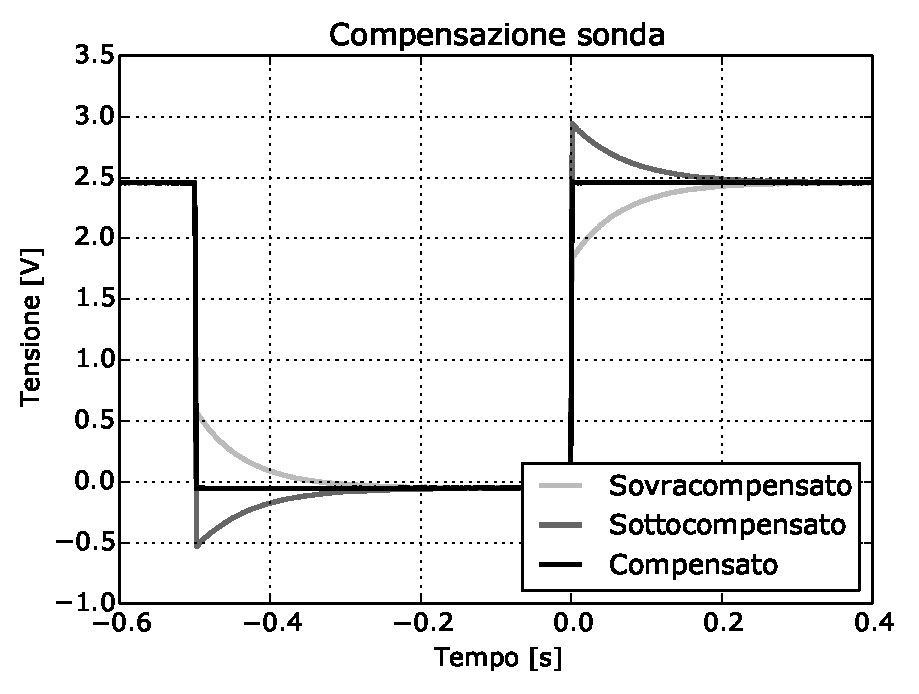
\includegraphics[width=\columnwidth]{figure/comp.pdf}
%    \caption{Input dell'oscilloscopio con una sonda compensabile. Cambiando capacità
%        si può ottenere una sottocompensazione, una sovracompensazione oppure compensare perfettamente
%        le capacità, ottenendo un'onda quadra.}
%    \label{fig:compensazione}
%\end{figure}

%\begin{wrapfloat}{figure}{O}{0pt}
%        \def\svgwidth{0.4\textwidth}
%        \subimport{figure/}{raddrizzatore.pdf_tex}
%        \caption{Raddrizzatore di precisione a semionda. Alimentato, inizialmente con una $V\ped{in}\,=\,\SI{1.02}{\volt}$ di frequenza $\nu\,=\,\SI{50}{\hertz}$.}
%        \label{fig:radd}
%\end{wrapfloat}

%\begin{SCfigure}[][p]
%        \centering
%        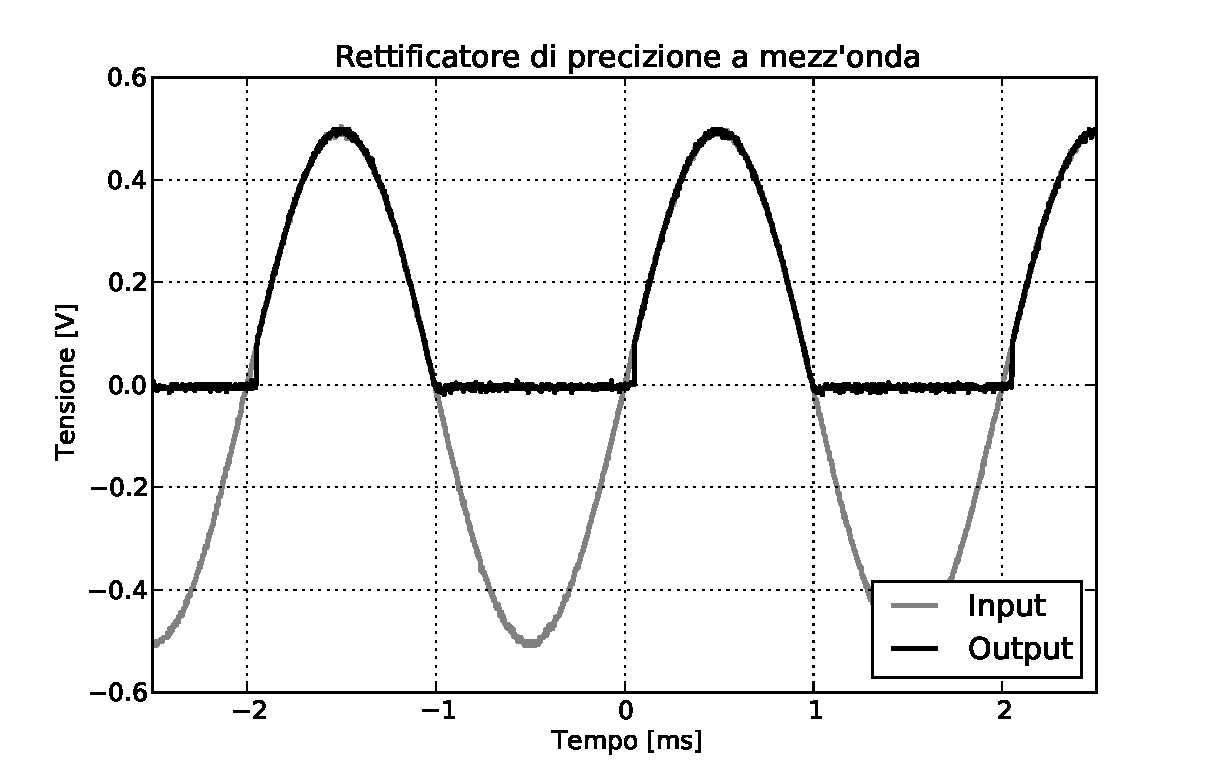
\includegraphics[width=0.7\textwidth]{figure/rett.pdf}
%        \caption{Questo grafico illustra l'andamento di $V\ped{out}$, linea nera, in funzione di $V\ped{in}$, linea grigia. Si nota chiaramente, come da previsioni, che la parte negativa del segnale in ingresso impediscse al diodo di condurre, pertanto la tensione di output risulta nulla. Inoltre, come si può osservare, il fronte di salita di $V\ped{out}$ presenta un leggero ritardo rispetto al segnale in ingresso $V\ped{in}$. Questo ritardo è stato stimato essere approssimativamente di circa $(152\pm10)\SI{}{\micro\second}$.}
%        \label{fig:radd_plot1}
%\end{SCfigure}
